\documentclass{article}

% Language setting
\usepackage[english, french]{babel}
\usepackage[T1]{fontenc} 
\usepackage[autolanguage]{numprint}

% Set page size and margins
\usepackage[a4paper,top=2cm,bottom=2cm,left=3cm,right=3cm,marginparwidth=1.75cm]{geometry}

% item
\usepackage{enumitem}

% Useful packages
\usepackage{amsmath,amssymb}
\usepackage{graphicx}
\usepackage[export]{adjustbox}
\usepackage[colorlinks=true, allcolors=blue]{hyperref}
\usepackage{multicol}
\usepackage{listings}
\usepackage{minted}

%\title{La Manipulation du Marché de l'Art}
%\title{Rapport DSB}
%\author{Florian EPAIN et Thomas De Premorel}
%\date{March 23, 2022}



\begin{document}

\begin{titlepage}
   \begin{center}
       \vspace*{1cm}
       \Huge
       \textbf{La Manipulation du Marché de l'Art}

       \vspace{0.5cm}
       \LARGE
        Rapport DSB
        
        \text{Groupe 2}
            
       \vspace{1.5cm}

       \textbf{Florian EPAIN}
       
       \text{florian.epain@etudiant.univ-rennes1.fr}
       
       \textbf{Thomas De Premorel}
       
       \text{???@etudiant.univ-rennes1.fr}
       
       \vspace{0.5cm}
       \text{March 23, 2022}

   \end{center}
   
   \vspace{13cm}
    \begin{abstract}
        C'est surement indigeste mais j'y ai mis mon coeur.
    \end{abstract}
\end{titlepage}



\tableofcontents
\clearpage

%%%%%%%%%%%%%%%%%%%%%%%%%%%%%%%%%%%%%%%%%%%%%%%%%%%%%%%%%%%%%%%%%%%%%%%%%%%%%%%%%%%%%%%%%%%%%%%%%%%%%%%%%%%%

\section{Introduction}

Nous avons choisi de représenter la 'discrimination' des artistes dans le marché de l'art et le principe d'évaluation d'une oeuvre d'art.

Depuis l'aube des temps, les artistes ont eu du mal à se rémunérer et ce phénomène est d'autant plus fort dans ce monde d'hyper-concurence et néocapitaliste.

D'après les dits de cette video : 
\begin{figure}[htp]
    \centering
    \href{https://www.youtube.com/watch?v=ZZ3F3zWiEmc}
    {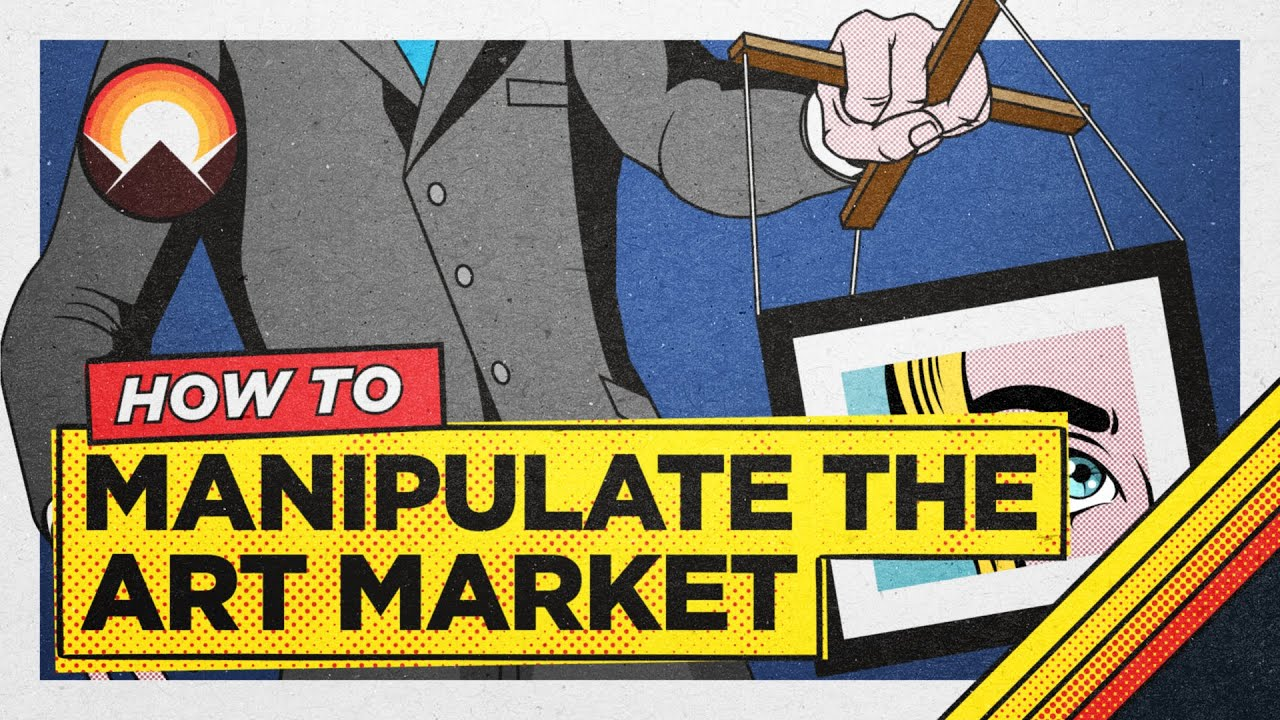
\includegraphics[width=0.5\textwidth]{miniature.jpeg}}
    \caption{\label{fig:miniature}The Art Market is a Scam (And Rich People Run It)}
\end{figure}

L'art n'a pas de valeur intrisèque.
L'art se voit etre évalué par la somme \emph{hypothétique} que les acheteurs \emph{potentiels} sont prêt à dépenser pour l'acquérir. Il en va donc d'une enchère monétaire, de manipulation de critique, mais aussi de recherche et de travaux d'expert sur certaines oeuvres pour que celle-ci se voit identifiée, voire authentifiée, ce qui a pour cause de monter son prix.
\\

Ce marché est très restreint, accessible uniquement par des strates très riches de nos sociétés. En effet, le prix d'entrée des marchés où se déroulent les ventes les plus 'lucratives' et onéreuses dépasse souvent le salaire moyen d'une vie d'un salarié (source dans un prochain épisode).

La grande majorité des ventes mondiales d'art sont concentrées à New york, Hong-kong et London.
\\

Le problème se pose sur le caractère spéculatif (stéril et fictif), subjectif et concentré de ce système. Ce sont dans ce genre de petit monde où le monopole contrôle tout (les prix, quand pour les ventes, combien d'oeuvre, etc) -> \href{https://youtu.be/ZZ3F3zWiEmc?t=895}{l'exemple} des oeuvres d'Andy Warhol et du presque unique acheteur Jose Mugrabi.

Ces mêmes conditions qu'a permit à Mugrabi de dominer le marché des oeuvres de Warhol, à son influence de fonctionner reflètent que la connivence et la corruption s'y confonde facilement.
\\

Nous parlons même pour le marché de l'art d'une composition d'arnaques, par exemple : \newline
Contre-intuitivement, d'ultra-riche individus peuvent gagner en rentabilité en procédant à des donations d'art.

    Pour le cas des US -se trouve également en France-, lorsqu'un de ces individus opère une donation d'art à un musée -à but non-lucratif- il obtient une déduction de taxe.
    
        Pour un don d'une oeuvre valant 10 millions de \$\, la déduction d'impôt s'applique pour 10 millions, qui en théorie devrait leur profiter de 4 millions.
    Etant donné la difficulté de determiner la valeur d'oeuvre, l'IRS (\href{https://www.irs.gov/}{Internal Revenue Service} : organisme de taxation des Etats Unis vis-à-vis de l'art) se voit surpayer 38\%\ des déductions de taxes comparement à la valeur établie plus tard. (source manquante dans la vidéo)
    
        En résumé, un ultra-riche pourrait acheter un pièce d'art pour 4millions.
        L'apprécier pendant quelque année, négocier pour une évaluation favorable, augmenter sa valeur, se baser sur le fait que l'IRS n'audite (ne contrôle) qu'une infime partie des oeuvres, faire la donation pour 10millions et il aura déjà atteint le seuil de rentabilité.
        
        Ce don aura également pour cause, la présence d'une piece d'une même collection dans le musée, d'augmenter le prix des autres de la collection que ce créancier possède potiellement (puissance d'un monopole).

\paragraph{L'art n'est plus un exercice de compétence, c'est celui d'une marque.}

%%%%%%%%%%%%%%%%%%%%%%%%%%%%%%%%%%%%%%%%%%%%%%%%%%%%%%%%%%%%%%%%%%%%%%%%%%%%%%%%%%%%%%%%%%%%%%%%%%%%%%%%%%%%

\section{Modèle conceptuel}


Nous avons omis les conservateurs de musée, propriétaire de gallerie et d'autres acteurs dans l'équation de l'évaluation du prix d'une oeuvre. 
Les relations de connaisance entre les différents humains, leur contact, leur société écran, \emph{etc.} 
Ce procédé reste complexe et non exhaustivement représenté par cette base de donnée.
Il s'agit surtout d'une ébauche.

\subsection{Description du modèle}

L'art est au milieu de tout ce système. 
Ce marché se compose de plusieurs acteurs, chacun influence la valeur de l'oeuvre.
Comme représenté sur ce shéma mocodo : \ref{fig:MCD_last}

Une pièce d'oeuvre d'art possède:
\begin{itemize}[label=\(\blacktriangleright\)]
    \item un numéro d'objet (unique);
    \item un titre;
    \item un medium (type);
    \item une cote (la valeur estimée de l'oeuvre).
\end{itemize}
Nous avons décidé de séparer le créateur de la pièce, étant donné que son créateur peut etre inconnu ou en avoir plusieurs.


\begin{multicols}{2}[]
Nombreuses tables représentent des humains, pour pouvoir les différencier nous les avons séparé en plusieurs tables.
Ces humains possèdent tous ces \emph{attributs fixes}:
\begin{itemize}[label=\(\blacktriangleright\)]
    \item un identifiant unique*;
    \item un nom;
    \item une nationalité.
\end{itemize}

Certains d'entre eux peuvent avoir comme attribut :
\begin{itemize}[label=\(\blacktriangleright\)]
    \item un capital;
    \item une spécialité;
    \item un site web;
    \item une réputation.
\end{itemize}
\end{multicols}


Les attributs des artistes sont tous facultatifs sauf leur identifiant qui lui est unique.
En effet, on va créer un profil artiste lorsqu'on retrouve une collection d'oeuvre à l'artiste inconnu, on les regroupe par un artiste 'fantôme'.
Ils possèdent potentiellement un site-web -un contact- et une réputation.
Cette réputation est positive, un artiste avec une réputation :
\begin{itemize}[label=\(\blacktriangleright\)]
    \item = 0 est inconnu;
    \item > 1000 est connu localement;
    \item > 2000 est connu à l'internationale;
    \item > 10000 est une figure historique.
\end{itemize}

On associe les artistes avec les artworks par la relation CREE.
Un Artwork peut etre créé par personne ou plusieurs artistes. Et un artiste peut ne rien avoir créé ou avoir une multitude de création.


Les Mecenes sont peu majoritaire dans le marche de l'art,
il s'agit surtout de créancier qui achetent directement à l'artiste. 
Ils possèdent les attributs humains fixes, une réputation (même ordre que celle des les artistes) et leur patrimoine supposé (capital).
Ces Mecènes peuvent ou pas AIDE un ou des artistes, représenté par une somme d'argent : montantAide 

    
\begin{multicols}{2}[]
Les Créanciers sont principalement des commerciaux plutôt que des collectionneurs d'art. 
Ils ont les attributs fixes et un capital.
Ils peuvent vendre de l'art, à un certain prix (prixVente), à un certain moment (dateDeVente).
Ils peuvent participer à un seul marché à la fois, dans lequel ils peuvent acheter/vendre des oeuvres répertoriée dans la relation PARTICIPE
Pour les achats de crénacier à créancier privé (sans marché public) on passe par possede.
\\ \\

Les Commissaires-priseurs ont seulement les attributs fixes.
Ils peuvent diriger un marché.

Pour qu'une oeuvre monte en valeur, et s'affiche mieux dans un immense salon,
les Restaurateurs travaillent avec les Musées, les galeries et les collectionneurs d'art (créancier).
Ils ont une spécialité (typeRestaurateur) sur laquelle ils travaillent un medium
Ils sont en contact direct avec les oeuvres (relation RESTAURE: pour un certain prix (prixRestauration)).
\\

    Les Critiques sont des personnes publiques émettant un jugement sur certaine oeuvre, mouvement d'art.
Ils jouent un rôle important dans la monter de prix des oeuvres (relation JUGE: en donnant une cote -coteDonnee-).
\end{multicols}

\clearpage

Enfin les Experts sont des chercheurs, en Histoire, en Matière, en Technique.
Leur collaboration avec le corps des galeries et créanciers est essentielle pour l'authentification d'oeuvre d'art.
Prouver qu'une pièce est l'original peut faire grimper sa cote de plusieurs millions. \cite{Christ's_Portrait}
\\

Le marché devra être dirigé par un commissaire-priseur et peut avoir aucun ou plusieurs créanciers participant.
Il s'agit de galerie privée, où le prix d'entrée (prixEntryMarche) vise à resteindre les acheteurs (n'avoir que la même 'clientèle').
Ils sont unique et ne durent que le jour dateMarche*.
Ces marchés peuvent être heberger par des organismes privés ou avoir des locaux fixes comme \href{https://fr.wikipedia.org/wiki/Christie's}{Christies's} ou \href{https://fr.wikipedia.org/wiki/Sotheby's}{Sotheby's}.
Il se déroule à un certain moment (dateMarche), rendez vous à ne pas manquer pour repérer les fluctuations de prix et certaines oeuvres qui peuvent se rentabiliser.
\\

Les Galeries et les Musées sont des organismes présentant des oeuvres (EXPOSE et PRET resp),
elles ne peuvent pas ouvrir si ces organismes n'ont pas assez d'oeuvres à exposer. 
(cardinalité N N).
Une oeuvre peut etre exposée / pretée plusieurs fois, pour garder l'historique.
Les attributs dureedebut / dureefin (dureedebutExpo/dureefinExpo et dureedebutPret/dureefinPret resp) correspond à deux DATEs entre laquelle la galerie ou le musée dispose de l'oeuvre.


\href{https://fr.wikipedia.org/wiki/Musée}{D'après l'ICOM}, un musée est une institution permanente sans but lucratif au service de la société et de son développement ouverte au public, qui acquiert, conserve, étudie, expose et transmet le patrimoine matériel et immatériel de l’humanité et de son environnement à des fins d'études, d'éducation et de délectation. 
Le musée doit avoir une dateCreation* et une adresseMusee*.

Une galerie à une date de creation ou date d'evenement pour les galeries temporaires (dateGalerie).
Un prixEntryExpo, pouvant dépassant les centaines de milliers de dollars.
Une galerie peut reverser les gains à une association. (smiley qui sourit)
Une galerie peut être à l'extérieur, à l'intérieur dans des locaux fixes ou mobiles.



%\begin{figure}[htp]
%\centering 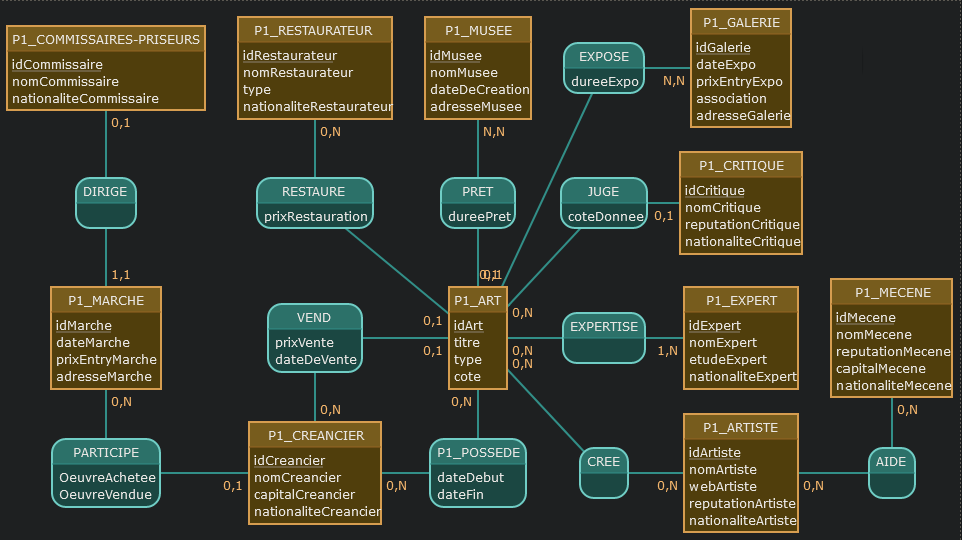
\includegraphics[width=1\textwidth]{mocodo_old.png} \caption{\label{fig:MCD_old}Ancien Schéma Mocodo.}
%\end{figure}

\begin{figure}[htp]
\centering
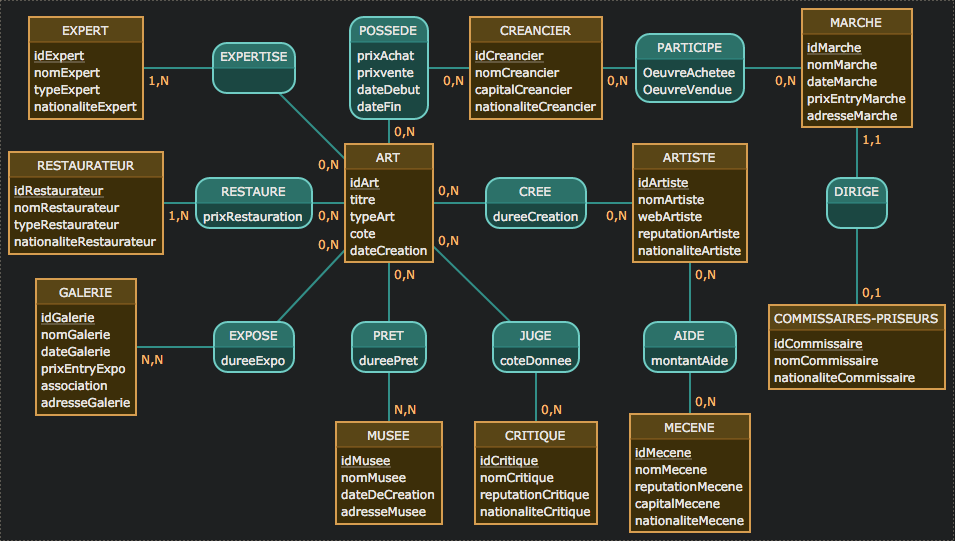
\includegraphics[width=1\textwidth]{new_mocodo.png}
\caption{\label{fig:MCD_last}Schéma Mocodo Revisité.}
\end{figure}


\clearpage

%%%%%%%%%%%%%%%%%%%%%%%%%%%%%%%%%%%%%%%%%%%%%%%%%%%%%%%%%%%%%%%%%%%%%%%%%%%%%%%%%%%%%%%%%%%%%%%%%%%%%%%%%%%%

\section{Modèle relationnel}
\subsection{Application règle 1}

ART ( \underline{idArt}, titre, typeArt, cote, dateCreation ) \newline
%pb : l'importation de la BDD MoMA met 0 à la place du vide pour bcp d'attrib
COMMISSAIRE-PRISEUR ( \underline{idCommissaire}, nomCommissaire*, nationaliteCommissaire )\newline
RESTAURATEUR ( \underline{idRestaurateur}, nomRestaurateur*, typeRestaurateur*, nationaliteRestaurateur )\newline
MUSEE ( \underline{idMusee}, nomMusee*, dateDeCreation*, adresseMusee )\newline
GALERIE ( \underline{idGalerie}, nomGalerie*, dateGalerie*, prixEntryExpo, association, adresseGalerie* )\newline
CRITIQUE ( \underline{idCritique}, nomCritique*, reputationCritique, nationaliteCritique )\newline
MARCHE ( \underline{idMarche}, nomMarche*, dateMarche*, prixEntryMarche, adresseMarche*)\newline
EXPERT ( \underline{idExpert}, nomExpert*, typeExpert*, nationaliteExpert )\newline
MECENE ( \underline{idMecene}, nomMecene*, reputationMecene, capitalMecene, nationaliteMecene )\newline
CREANCIER ( \underline{idCreancier}, nomCreancier*, capitalCreancier, nationaliteCreancier )\newline
ARTISTE ( \underline{idArtiste}, nomArtiste, webArtiste, reputationArtiste, nationaliteArtiste )\newline

\subsection{Application règle 2 et 2bis}

Les 0 1 et 1 1 se transforment en clé étrangères et supprime la relation qui est alors inutile.
Ici le marché étant unique, il n'est dirigé que par un seul commissaire-priseur, la relation dirige est alors incorporée dans la table marché.

MARCHE ( \underline{idMarche}, nomMarche*, dateMarche*, prixEntryMarche, adresseMarche*, \underline{\underline{idcommissaire}})

\subsection{Application règle 3}

Ces relations deviennent des tables contenant des clés étrangères pour permettre à toutes informations de pouvoir être accèder sans ambiguité.
Et les relations inutiles sont supprimées 
\\
PARTCIPE(\underline{\underline{idMarche}}*, \underline{\underline{idCreancier}}*)
\\
POSSEDE(\underline{\underline{idCreancier}}*, \underline{\underline{idArt}}*, prixAchat, prixVente, dateDebutPossede*, dateFinPossede) \newline

Les deux relation POSSEDE et VEND sont fusionné afin d'éviter les conflits \newline
Le prix peut etre privé (sans trop d'interet dans le milieu de la spéculation) \newline
\\
RESTAURE(\underline{\underline{idRestaurateur}}*, \underline{\underline{idArt}}*, prixRestaure) \newline
PRET(\underline{\underline{idMusee}}*, \underline{\underline{idArt}}*, dureedebutPret*, dureefinPret*) \newline
EXPOSE(\underline{\underline{idGalerie}}*, \underline{\underline{idArt}}*, dureedebutExpose*, dureefinExpose*) \newline
JUGE(\underline{\underline{idCritique}}*, \underline{\underline{idArt}}*, prixJuge*) \newline
EXPERTISE(\underline{\underline{idExpert}}*, \underline{\underline{idArt}}*) \newline
CREE(\underline{\underline{idArtiste}}*, \underline{\underline{idArt}}*) \newline
AIDE(\underline{\underline{idMecene}}*, \underline{\underline{idArtiste}}*, prixAide) \newline


\clearpage

\newgeometry{left=0.5cm,right=0.5cm,top=0.5cm,bottom=1.5cm}

\section{Schéma physique}

\begin{multicols}{2}


\begin{minted}
{sql}
CREATE DATABASE IF NOT EXISTS `MERISE`
DEFAULT CHARACTER SET utf8
COLLATE utf8_general_ci;
USE `MERISE`;
DROP TABLE IF EXISTS POSSEDE;
DROP TABLE IF EXISTS CREE;
DROP TABLE IF EXISTS PARTICIPE;
DROP TABLE IF EXISTS EXPOSE;
DROP TABLE IF EXISTS RESTAURE;
DROP TABLE IF EXISTS PRET;
DROP TABLE IF EXISTS JUGE;
DROP TABLE IF EXISTS EXPERTISE;
DROP TABLE IF EXISTS AIDE;
DROP TABLE IF EXISTS CRITIQUE;
DROP TABLE IF EXISTS EXPERT;
DROP TABLE IF EXISTS ARTISTE;
DROP TABLE IF EXISTS MECENE;
DROP TABLE IF EXISTS RESTAURATEUR;
DROP TABLE IF EXISTS MUSEE;
DROP TABLE IF EXISTS GALERIE;
DROP TABLE IF EXISTS ART;
DROP TABLE IF EXISTS CREANCIER;
DROP TABLE IF EXISTS MARCHE;
DROP TABLE IF EXISTS COMMISSAIRE_PRISEUR;

CREATE TABLE ART (
  idart INT NOT NULL,
  titre VARCHAR(1000),
  typeArt VARCHAR(1000),
  cote VARCHAR(1000),
  dateCreation VARCHAR(1000),
  PRIMARY KEY (idart)
);

CREATE TABLE ARTISTE (
  idartiste INT NOT NULL,
  nomartiste VARCHAR(1000),
  webartiste VARCHAR(1000),
  reputationartiste INT,
  nationaliteartiste VARCHAR(1000),
  PRIMARY KEY (idartiste)
);

CREATE TABLE COMMISSAIRE_PRISEUR (
  idcommissaire INT NOT NULL,
  nomcommissaire VARCHAR(1000) NOT NULL,
  nationalitecommissaire VARCHAR(1000),
  PRIMARY KEY (idcommissaire)
);

CREATE TABLE MARCHE (
  idmarche INT NOT NULL,
  nommarche VARCHAR(1000) NOT NULL,
  datemarche DATE NOT NULL,
  prixentrymarche VARCHAR(1000),
  adressemarche VARCHAR(1000) NOT NULL,
  idcommissaire INT NOT NULL,
  PRIMARY KEY (idmarche),
  FOREIGN KEY (idcommissaire)
  REFERENCES COMMISSAIRE_PRISEUR(idcommissaire)
);


CREATE TABLE RESTAURATEUR (
  idrestaurateur INT NOT NULL,
  nomrestaurateur VARCHAR(1000) NOT NULL,
  typerestaurateur VARCHAR(100) NOT NULL,
  nationaliterestaurateur VARCHAR(42),
  PRIMARY KEY (idrestaurateur)
);

CREATE TABLE MUSEE (
  idmusee INT NOT NULL,
  nommusee VARCHAR(1000) NOT NULL,
  datemusee DATE NOT NULL,
  prixentrymusee INT,
  adressemusee VARCHAR(1000) NOT NULL,
  PRIMARY KEY (idmusee)
);

CREATE TABLE GALERIE (
  idgalerie INT NOT NULL,
  nomgalerie VARCHAR(1000) NOT NULL,
  dategalerie DATE NOT NULL,
  prixentrygalerie INT,
  association VARCHAR(1000),
  adressegalerie VARCHAR(1000) NOT NULL,
  PRIMARY KEY (idgalerie)
);

CREATE TABLE CRITIQUE (
  idcritique INT NOT NULL,
  nomcritique VARCHAR(1000) NOT NULL,
  reputationcritique INT,
  nationalitecritique VARCHAR(1000),
  PRIMARY KEY (idcritique)
);

CREATE TABLE EXPERT (
  idexpert INT NOT NULL,
  nomexpert VARCHAR(1000) NOT NULL,
  typeexpert VARCHAR(1000) NOT NULL,
  nationaliteexpert VARCHAR(1000),
  PRIMARY KEY (idexpert)
);

CREATE TABLE MECENE (
  idmecene INT NOT NULL,
  nommecene VARCHAR(1000) NOT NULL,
  reputationmecene INT,
  capitalmecene INT,
  nationalitemecene VARCHAR(1000),
  PRIMARY KEY (idmecene)
);

CREATE TABLE CREANCIER (
  idcreancier INT NOT NULL,
  nomcreancier VARCHAR(1000) NOT NULL,
  capitalcreancier INT,
  nationalitecreancier VARCHAR(1000),
  PRIMARY KEY (idcreancier)
);





CREATE TABLE POSSEDE (
  idcreancier INT NOT NULL,
  idart INT NOT NULL,
  prixAchat INT,
  prixVente INT,
  datedebutPossede DATE NOT NULL,
  datefinPossede DATE,
  PRIMARY KEY (idcreancier, idart),
  FOREIGN KEY (idart)
  REFERENCES ART(idart),
  FOREIGN KEY (idcreancier)
  REFERENCES CREANCIER(idcreancier)
);

CREATE TABLE CREE (
  idartiste INT NOT NULL,
  idart INT NOT NULL,
  PRIMARY KEY (idartiste, idart),
  FOREIGN KEY (idart)
  REFERENCES ART(idart),
  FOREIGN KEY (idartiste)
  REFERENCES ARTISTE(idartiste)
);

CREATE TABLE PARTICIPE (
  idcreancier INT NOT NULL,
  idmarche INT NOT NULL,
  PRIMARY KEY (idcreancier, idmarche),
  FOREIGN KEY (idcreancier)
  REFERENCES CREANCIER(idcreancier),
  FOREIGN KEY (idcreancier)
  REFERENCES MARCHE(idmarche)
);

CREATE TABLE EXPOSE (
  idart INT NOT NULL,
  idgalerie INT NOT NULL,
  dureedebutexpose DATE NOT NULL,
  dureefinexpose DATE NOT NULL,
  PRIMARY KEY (idart, idgalerie),
  FOREIGN KEY (idart)
  REFERENCES ART(idart),
  FOREIGN KEY (idgalerie)
  REFERENCES GALERIE(idgalerie)
);









CREATE TABLE RESTAURE (
  idrestaurateur INT NOT NULL,
  idart INT NOT NULL,
  prixrestaure INT,
  PRIMARY KEY (idrestaurateur, idart),
  FOREIGN KEY (idart)
  REFERENCES ART(idart),
  FOREIGN KEY (idrestaurateur)
  REFERENCES RESTAURATEUR(idrestaurateur)
);

CREATE TABLE PRET (
  idart INT NOT NULL,
  idmusee INT NOT NULL,
  dureedebutpret DATE NOT NULL,
  dureefinpret DATE NOT NULL,
  PRIMARY KEY (idart, idmusee),
  FOREIGN KEY (idart)
  REFERENCES ART(idart),
  FOREIGN KEY (idmusee)
  REFERENCES MUSEE(idmusee)
);

CREATE TABLE JUGE (
  idcritique INT NOT NULL,
  idart INT NOT NULL,
  prixJuge INT NOT NULL,
  PRIMARY KEY (idcritique, idart),
  FOREIGN KEY (idart)
  REFERENCES ART(idart),
  FOREIGN KEY (idcritique)
  REFERENCES CRITIQUE(idcritique)
);

CREATE TABLE EXPERTISE (
  idexpert INT NOT NULL,
  idart INT NOT NULL,
  PRIMARY KEY (idexpert, idart),
  FOREIGN KEY (idart)
  REFERENCES ART(idart),
  FOREIGN KEY (idexpert)
  REFERENCES EXPERT(idexpert)
);

CREATE TABLE AIDE (
  idmecene INT NOT NULL,
  idartiste INT NOT NULL,
  prixAide INT,
  PRIMARY KEY (idmecene, idartiste),
  FOREIGN KEY (idartiste)
  REFERENCES ARTISTE(idartiste),
  FOREIGN KEY (idmecene)
  REFERENCES MECENE(idmecene)
);
\end{minted}
\end{multicols}

\restoregeometry

\section{Peuplement des tables uwu}

\href{https://github.com/MuseumofModernArt/collection}{Github: Museum of Modern Art}

Nous avons utilisé seulement quelque informations contenues dans la base de données MoMA :
\\Pour les artistes :
\begin{itemize}[label=\(\blacktriangleright\)]
    \item DisplayName (leur nom);
    \item Nationality (leur origine).
\end{itemize}
Pour les oeuvres d'art :
\begin{itemize}[label=\(\blacktriangleright\)]
    \item Title;
    \item Artist;
    \item Medium;
    \item Date de création.
\end{itemize}

Toutes les autres informations contenues dans notre base de données
n'est que pure supposition et imagination (cote d'une oeuvre / reputation d un artiste / \emph{etc})


\subsection{Artistes}

On importe depuis le .json du MoMA, la table artiste contenant 133038 individus/organismes.
On utilise le code convert\_artists() (\hyperref[sec:convArtists]{section 7.1})
Deux exemples d'artiste : 
\begin{minted}
[
frame=lines,
framesep=2mm,
%baselinestretch=1.2,
%bgcolor=LightGray,
%fontsize=\footnotesize,
linenos
]
{json}
{
  "constituent_id": 7626,
  "display_name": "Patrick Ireland",
  "artist_bio": "Irish, 1972–2008",
  "nationality": "Irish",
  "gender": "Male",
  "begin_date": 1972,
  "end_date": 2008,
  "wiki_qid": "Q3777954",
  "ulan": "500079431"
},

{
  "constituent_id": 7636,
  "display_name": "IBM Corporation",
  "artist_bio": "American, founded 1911",
  "nationality": "American",
  "gender": null,
  "begin_date": 1911,
  "end_date": 0,
  "wiki_qid": null,
  "ulan": null
},
\end{minted}


\subsection{Artworks}

On importe depuis le .json du MoMA, la table artwork contenant 419289 pièces d'art.
On utilise le code convert\_artworks() (\hyperref[sec:convArtworks]{section 7.2})
Toutes les dates vont etre à 0 ou null car la base de donnée MoMA insere des phrases (Option<String>) dans l'attribut date de l'artwork.

\newgeometry{left=1cm,right=0.5cm,top=0.5cm,bottom=1.5cm}
Un exemple d'artwork : 
\begin{minted}
[
frame=lines,
framesep=2mm,
%baselinestretch=1.2,
%bgcolor=LightGray,
%fontsize=\footnotesize,
linenos
]
{json}
{
  "title": "Zamaul' III",
  "artist": [
    "Various artists",
    "Vladimir Burliuk",
    "Pavel Filonov",
    "Aleksei Kruchenykh",
    "Il'ia Rogovin"
  ],
  "constituent_id": [
    24409,
    12001,
    12124,
    3263,
    23615
  ],
  "artist_bio": [
    "Ukrainian, 1886–1917",
    "Russian, 1883–1941",
    "Russian, 1886–1969"
  ],
  "nationality": [
    "",
    "Ukrainian",
    "",
    "Russian"
  ],
  "begin_date": [
    0,
    1886,
    1883,
    1886,
    0
  ],
  "end_date": [
    0,
    1917,
    1941,
    1969,
    0         ],
  "gender":   [
    "",
    "Male",
    "Male",
    "Male",
    "Female" ],
  "date": "1919",
  "medium": "Book with five hectographed illustrations,
  letterpress and rubber-stamped typographic designs, and hectographed manuscript text and designs",
  "dimensions": "page (irreg.): 6 1/2 x 5 13/16\ (16.5 x 14.8 cm)",
  "credit_line": "Gift of The Judith Rothschild Foundation",
  "accession_number": "114.2001",
  "classification": "Illustrated Book",
  "department": "Drawings & Prints",
  "date_acquired": "2001-01-24",
  "cataloged": "Y",
  "object_id": 11384,
  "url": "http://www.moma.org/collection/works/11384",
  "thumbnail_url": "http://www.moma.org/media/W1siZiIsIjIxMjY5NCJdLFsicCIsImNvbnZlcnQiLCItcmVzaXplIDMwMHgzMDBcdTAwM2UiXV0.jpg?sha=7193a69ce29794bf",
  "height_cm": 16.5,
  "width_cm": 14.8
},
\end{minted}

\restoregeometry

\subsection{Humains}

À partir d'ici, nous n'avons plus de base de donnée à importer alors nous allons créer des humains.

On créé deux tableaux contenant des prénoms et noms.

\begin{minted}
[
frame=lines,
framesep=2mm,
%baselinestretch=1.2,
%bgcolor=LightGray,
%fontsize=\footnotesize,
linenos
]
{rust}
static LIST_FIRST_NAME: &'static [&str] = &["Adrien", "Nelson", "Benoit", "Morgan",
"Florian", "Thomas", "Maeto", "Clementine", "Stephane", "Otto", "Jan", "Patrick",
"Rudolf", "Pietra", "Lex", "Nancy", "Waltercio", "Peter", "George", "Jotaro",
"Joseph", "Jonathan", "Joe", "Maria", "Laurence", "Emil", "Usul", "Wout", "Montse",
"Bent", "Nobert", "Marcel", "Arian", "Hella"];

static LIST_LAST_NAME: &'static [&str] = &["Strömholm", "Strömholm", "Rusten",
"Russomagno", "Biddle", "Burckhardt", "Martin", "Pinney", "Neusüss", "Goldes",
"Charlesworth", "Bernsten", "Appelt", "Cohen", "McCarthy", "Wagner", "Van Toorn",
"Mol", "Lynch", "Bell", "Cassell", "Schönthal", "Kammerer", "Hoppe", "De Vringer",
"Faydherbe", "Marqués", "Nobert", "Smith", "Knoll", "Rizzatto", "Tetrarc",
"Wanders", "van der Meulen", "Joestar", "Abitbol", "Zepelli", "Speedwagon"];
\end{minted}

On importe depuis le .json artistes un tableau pour l'origine (de leur attribut nationality):
\begin{minted}
[
frame=lines,
framesep=2mm,
%baselinestretch=1.2,
%bgcolor=LightGray,
%fontsize=\footnotesize,
linenos
]
{rust}
static LIST_NATIONALITY: &'static [&str] = &["nationality unknown", "American",
"Spanish", "Danish", "Italian", "French", "Estonian", "Mexican", "Swedish",
"Israeli", "British", "Finnish", "Polish", "Palestinian", "Japanese", "Guatemalan",
"Colombian", "Romanian", "Russian", "German", "Argentine", "Kuwaiti", "Belgian",
"Dutch", "Norwegian", "Chilean", "Swiss", "Costa Rican", "Czech", "Brazilian",
"Austrian", "Canadian", "Australian", "Ukrainian", "Hungarian", "Haitian",
"Congolese", "Bolivian", "Cuban", "Yugoslav", "Portuguese", "Indian", "Peruvian",
"Icelandic", "Irish", "Guyanese", "Uruguayan", "Slovak", "Croatian", "Greek",
"Chinese", "Venezuelan", "Turkish", "Panamanian", "Algerian", "Ecuadorian",
"South African", "Iranian", "Korean", "Canadian Inuit", "Paraguayan",
"Luxembourgish", "Nicaraguan", "Zimbabwean", "Moroccan", "Slovenian", "Tanzanian",
"Bulgarian", "Tunisian", "Sudanese", "Taiwanese", "Ethiopian", "Scottish",
"Latvian", "Senegalese", "Thai", "New Zealander", "Lithuanian", "Pakistani",
"Bahamian", "Bosnian", "Malian", "Czechoslovakian", "Georgian", "Egyptian",
"Kenyan", "Emirati", "Nigerian", "Cypriot", "Albanian", "Azerbaijani", "Ivorian",
"Malaysian", "Serbian", "Singaporean", "Namibian", "Cambodian", "Ghanaian",
"Afghan", "Native American", "Lebanese", "Kyrgyzstani", "Vietnamese", "Ugandan",
"Cameroonian", "Welsh", "Macedonian", "Puerto Rican", "Catalan", "Filipino",
"Sahrawi", "Bangladeshi", "Coptic", "Persian", "Burkinabe", "Beninese",
"Sierra Leonean", "Salvadoran"];
\end{minted}

On créé un tableau pour les différents types globaux de medium.
\begin{minted}
[
frame=lines,
framesep=2mm,
%baselinestretch=1.2,
%bgcolor=LightGray,
%fontsize=\footnotesize,
linenos
]
{rust}
static LIST_ARTWORK_TYPE: &'static [&str] = &["Sculture", "Paint", "Ceramics",
"Graphic Art", "Illuminated Manuscripts", "Jewellery Art", "Metalwork Art",
"Mosaic Art", "Photography", "Architecture", "Religious Art", "Rock Art",
"Stained Glass Art"];
\end{minted}

On crée une multitude de methodes pour décrire tous les attributs des humains (\hyperref[sec:createAttr]{section 7.3}).
On crée une méthode pour générer et insérer des humains (\hyperref[sec:insHumans]{section 7.4}).

Un exemple d'appel pour créer amounth\_of\_each créanciers : 
\begin{minted}
[
frame=lines,
framesep=2mm,
%baselinestretch=1.2,
%bgcolor=LightGray,
%fontsize=\footnotesize,
linenos
]
{rust}

pub fn create_requests(amount_of_each: i32) // -> Result<()>
{
    let mut request: String = "".to_string();

    let mut number_of_creation: i32 = 0;
    let creancier = create_insert_humans("creancier", amount_of_each, false, false, true);
    number_of_creation +=amount_of_each;
    request.push_str(&creancier);
    
    println!("humans created: {}", number_of_creation);
    println!("--------create_.txt---------");

    fs::write("E:/Code/projects_rust/art-manipulation/RENDU/humans.txt", request)
        .expect("Unable to write file");
\end{minted}

\subsection{Organismes}

Pour les organisations : Marché, Galerie, Musée.
Nous utilisons les mêmes méthodes attributs (\hyperref[sec:createAttr]{section 7.3}).

Le tableau (vide) qui peut contenir des associations (pour attr de galerie) :
\begin{minted}
[
frame=lines,
framesep=2mm,
%baselinestretch=1.2,
%bgcolor=LightGray,
%fontsize=\footnotesize,
linenos
]
{rust}
static LIST_ASSOCIATION: &'static [&str] = &["", ""];
\end{minted}

Pour insérer les organismes on utilise le code en \hyperref[sec:insOrg]{section 7.5}

\subsection{Relations}

On utilise les codes de la \hyperref[sec:createRel]{Section 7.6}
pour générer des fausses relations.

Deux exemple de création de relations :

\begin{minted}
[
frame=lines,
framesep=2mm,
%baselinestretch=1.2,
%bgcolor=LightGray,
%fontsize=\footnotesize,
linenos
]
{rust}
pub fn create_requests(amount_of_each: i32) // -> Result<()>
{
    let mut request: String = "".to_string();

    let mut number_of_creation: i32 = 0;
    
    //--POSSEDE------------------------------------------------------------------
    let own = create_possede("possede".to_string(), "creancier".to_string(),
                             "art".to_string(), amount_of_each, 2);
    number_of_creation +=amount_of_each;
    request.push_str(&own);

    //--RESTAURE-----------------------------------------------------------------
    let restore = create_insert_relations("restaure".to_string(), "restaurateur".to_string(),
                               "art".to_string(), amount_of_each, 18, true, false);
    number_of_creation +=amount_of_each;
    request.push_str(&restore);
    
    println!("inserts created: {}", number_of_creation);
    println!("--------create_.sql---------");

    fs::write("E:/Code/projects_rust/art-manipulation/RENDU/insertsFictiv.sql", request)
        .expect("Unable to write file");
}
\end{minted}

\section{Requetes SQL}

\subsection{Projection}


\subsection{Jointure}

\subsection{Moyenne sur l'integralite d'un attribut}

\subsection{Regroupement par calcul}

\subsection{Différence}

\subsection{Division}

\subsection{Group By}

\clearpage

\section{Code}

\subsection{convert\_artists()}
\label{sec:convArtists}
\begin{minted}
[
frame=lines,
framesep=2mm,
%baselinestretch=1.2,
%bgcolor=LightGray,
%fontsize=\footnotesize,
linenos
]
{rust}

#[derive(Serialize, Deserialize, Debug)]
struct Artist {
	constituent_id: i128,
	display_name: String,
	artist_bio: Option<String>,
	nationality: Option<String>,
	gender: Option<String>,
	begin_date: i16,
	end_date: i16,
	wiki_qid: Option<String>, 
	ulan: Option<String>
}

fn convert_artists() -> Result<()>
{
    let path = "E:/Code/projects_rust/MoMA/Artworks-reformed.json";

    let content = fs::read_to_string(path)
        .expect("Unable to read file");

    println!("-----read_.json-----");
	
    let artists: Vec<Artist> = serde_json::from_str(&content).unwrap();

    println!("--------create_request---------");

    let mut foo =
    "INSERT INTO P1_ARTISTE
    (idartiste, nomartiste, webartiste, reputationartiste, nationaliteartiste)
    \n VALUES ".to_string();

    for artist in artists
    {
        let artist_nationality: &str=
		match &artist.nationality {
			Some(s) => s,
			None => "",
		};


        let mut artist_web = artist.display_name
            .replace(" ", ".")
            .replace("'", "")
            .replace(",","");
        artist_web.push_str(".org");

        let foobar =
        "\n (id,'display_name','site', reputation,'nationality')";
        let mut artist_n = foobar.replace("id", &artist.constituent_id.to_string());
        artist_n = artist_n.replace("display_name", &artist.display_name.replace("'", " "));
        artist_n = artist_n.replace("site", &artist_web);
        artist_n = artist_n.replace("reputation",
                            &create_fictional_human::create_reputation(0,0).to_string());
        artist_n = artist_n.replace("nationality", &artist_nationality.replace("'", " "));
        foo.push_str(&artist_n);
        
        foo.push(','); // have to remove the last one
    }
    
    foo.push_str(";END"); //to end the SQL request
    foo = foo.replace(",;END",";");

    println!("--------create_.sql---------");

    fs::write("E:/Code/projects_rust/art-manipulation/RENDU/insert_artists.sql", foo)
        .expect("Unable to write file");

    Ok(())
}

\end{minted}

\subsection{convert\_artworks()}
\label{sec:convArtworks}

\begin{minted}
[
frame=lines,
framesep=2mm,
%baselinestretch=1.2,
%bgcolor=LightGray,
%fontsize=\footnotesize,
linenos
]
{rust}

fn convert_artworks() -> Result<()>
{
    let path = "E:/Code/projects_rust/MoMA/Artworks-reformed.json";
	let content = fs::read_to_string(path)
		.expect("Unable to read file");

	println!("-----read_.json-----");
	
    let artworks: Vec<Artwork> = serde_json::from_str(&content).unwrap();

	// println!("{:?}", artists);

	println!("--------create_request---------");

    let mut foo =
    "INSERT INTO P1_ART (idart, titre, typeArt, cote, dateCreation)
    \n VALUES ".to_string();

    for artwork in artworks
    {
        let artwork_medium: &str =
        match &artwork.medium {
            Some(s) => s,
            None => "",
        };

        let artwork_date: &str =
        match &artwork.date {
            Some(s) => {
                s.to_string().push_str("-01-01");
                s
            },
            None => "",
        };

        let artwork_title = artwork.title.replace("'", " ");

        //TODO : find potential ' and replace them by a space

        let foobar =
        "\n (id,'title', 'medium', cote)"; //, date)";
        let mut artwork_n = foobar.replace("id", &artwork.object_id.to_string());
        artwork_n = artwork_n.replace("title", &artwork_title.replace("\\", ""));
        // how on earth you can accept '\' in a user insertion... 
        artwork_n = artwork_n.replace("medium", &artwork_medium.replace("'", " ").replace("\\", ""));
        artwork_n = artwork_n.replace("cote", &create_fictional_human::create_reputation(0,0).to_string());
        // artwork_n = artwork_n.replace("date", &artwork_date.to_string());
        foo.push_str(&artwork_n);

        foo.push(','); // have to remove the last one
    }
    
    foo.push_str(";END"); //to end the SQL request
    foo = foo.replace(",;END",";");

    println!("--------create_.sql---------");

    fs::write("E:/Code/projects_rust/art-manipulation/Part1/indv/insert_artworks.sql", foo)
        .expect("Unable to write file");

    Ok(())
}

\end{minted}

\subsection{create all kind of attributes}
\label{sec:createAttr}
\begin{minted}
[
frame=lines,
framesep=2mm,
%baselinestretch=1.2,
%bgcolor=LightGray,
%fontsize=\footnotesize,
linenos
]
{rust}
pub fn create_reputation(_number_of_creation: i32, _base_reput: i32)->i32 {
    let mut rng = thread_rng();
    return rng.gen_range(1..2000);
}

fn create_name() -> String {
    let mut rng = thread_rng();

    let mut first_name: String =
        match &LIST_FIRST_NAME.choose(&mut rng) {
        Some(n) => n.to_string(),
            None => "Foo".to_string()
        };
    let last_name: String =
        match &LIST_LAST_NAME.choose(&mut rng) {
            Some(n) => n.to_string(),
            None => "Bar".to_string()
        };

    first_name.push_str(" ");
    first_name.push_str(&last_name);

    first_name
}

fn create_nationality() -> String {
    let mut rng = thread_rng();

    let nationality =
        match &LIST_NATIONALITY.choose(&mut rng) {
            Some(n) => n,
            None => "nationality unknown"
        };
    
    nationality.to_string()
}

fn create_type() -> String {
    let mut rng = thread_rng();

    let art_type: String = 
        match &LIST_ARTWORK_TYPE.choose(&mut rng) {
            Some(n) => n.to_string(),
            None => "Undefined".to_string()
        };

    art_type
}

fn create_capital() -> i128 {
    let mut rng = thread_rng();
    
    let capital: i128 = rng.gen_range(1..5000000)+1000000;

    capital
}

/**
 * @param past : 'a future date' -> false | 'a past date' -> true
 * format : AAAA-MM-JJ
 */
fn create_date(past: bool) -> String{
    let mut rng = thread_rng();

    let mut date = "year-month-day".to_string();
    let day = rng.gen_range(0..31); // dc about 31/02 or 31/04
    let month = rng.gen_range(0..12);
    let year; //= 1445;
    if past {
        year = rng.gen_range(2003..2021);
    }
    else {
        year = rng.gen_range(2022..2030);
    }
    
    date = date.replace("day", &day.to_string());
    date = date.replace("month", &month.to_string());
    date = date.replace("year", &year.to_string());

    date.to_string()
}

fn create_price() -> i32{
    let mut rng = thread_rng();
    // placeholder
    let price: i32 = rng.gen_range(0..50000);
    price
}

fn create_association() -> String{
    let mut rng = thread_rng();

    let association: String = 
        match &LIST_ASSOCIATION.choose(&mut rng) {
            Some(n) => n.to_string(),
            None => "Undefined".to_string()
        };

    association
}
\end{minted}

\subsection{create\_insert\_humans()}
\label{sec:insHumans}

\begin{minted}
[
frame=lines,
framesep=2mm,
%baselinestretch=1.2,
%bgcolor=LightGray,
%fontsize=\footnotesize,
linenos
]
{rust}
/**
 * create a sql request  to insert a good amount of data in your database
 * respect my current sql structure
 * should be great to import a example of struct with all table to auto all of this
 */
fn create_insert_humans(table_name: &str, amount: i32, art_type: bool,
                  reputation: bool, capital: bool) -> String 
{
    let mut request: String =
    "INSERT INTO P1_NAME (idname, nomname, "
        .to_string();
    if art_type {
        request.push_str("typename, ");
    }
    if reputation {
        request.push_str("reputationname, ");
    }
    if capital {
        request.push_str("capitalname, ");
    }
    
    request.push_str("nationalitename) \n VALUES");
    request = request
        .replace("NAME", &table_name.to_uppercase())
        .replace("name", &table_name.to_lowercase());

    for i in 0..amount {

        let name = create_name();

        let nationality = create_nationality();

        let foobar =
        "\n (id, 'display_name', ".to_string();

        let mut human_n = foobar.replace("id", &i.to_string());
        human_n = human_n.replace("display_name", &name);

        if art_type{
            human_n.push_str("'type', ");
            human_n = human_n.replace("type", &create_type());
        }
        if reputation{
            human_n.push_str("reputation, ");
            human_n = human_n.replace("reputation", &create_reputation(0,0).to_string());
        }
        if capital{
            human_n.push_str("capital, ");
            human_n = human_n.replace("capital", &create_capital().to_string());
        }

        human_n.push_str("'nationality'),");
        human_n = human_n.replace("nationality", &nationality);
        
        request.push_str(&human_n);

    }

    request.push_str(";END");
    request = request.replace(",;END","; \n \n");

    request
}
\end{minted}

\subsection{create\_insert\_organisations()}
\label{sec:insOrg}

\begin{minted}
[
frame=lines,
framesep=2mm,
%baselinestretch=1.2,
%bgcolor=LightGray,
%fontsize=\footnotesize,
linenos
]
{rust}
/**
 * if creation_date and rdv_date are true only creation_date will effect
 * you can't bassicaly have those two attributs
 */
fn create_insert_organisations(table_name: String, amount: i32, creation_date: bool,
                       rdv_date: bool, price: bool, association: bool) -> String
{
    let mut request: String =
    "INSERT INTO P1_NAME (idname, nomname, "
        .to_string();
    if creation_date {
        request.push_str("datedecreation, ");
    }
    // careful about this else which can conflict
    // with future change on mocodoStructre
    else if rdv_date { 
        request.push_str("datename, ");
    }
    if price {
        request.push_str("prixentryname, ");
    }
    request.push_str("adressename) \n VALUES");
    request = request
        .replace("NAME", &table_name.to_uppercase())
        .replace("name", &table_name.to_lowercase());

    for i in 0..amount {

        let name = create_name();

        let country = create_nationality();

        let foobar =
        "\n (id, 'display_name', ".to_string();

        let mut orga_n = foobar.replace("id", &i.to_string());
        orga_n = orga_n.replace("display_name", &name);
        if creation_date | rdv_date {
            //if rdv_date means !creation_date
            
            orga_n.push_str("date, ");   // same care here
            orga_n = orga_n.replace("date", &create_date(creation_date));
        }
        if price{
            orga_n.push_str("price, ");
            orga_n = orga_n.replace("price", &create_price().to_string());
        }
        if association{
            orga_n.push_str("association, ");
            orga_n = orga_n.replace("association", &create_association());
        }
        orga_n.push_str("'country'),");
        orga_n = orga_n.replace("country", &country);
        
        request.push_str(&orga_n);
    }

    request.push_str(";END");
    request = request.replace(",;END","; \n \n");

    request
}
\end{minted}

\subsection{create\_insert\_relations()}
\label{sec:createRel}

I didn't manage to merge the possede and the other methods together,
so there are two different methods.
\begin{minted}
[
frame=lines,
framesep=2mm,
%baselinestretch=1.2,
%bgcolor=LightGray,
%fontsize=\footnotesize,
linenos
]
{rust}
/**
 * frequence: if 0 -> no condition whatsoever (no filter),
 *            if 8 -> condition 1/8 (only 1/8 will be associate)
 * don't handle insert attributefor POSSEDE and PARTICIPE
 */
fn create_insert_relations(relation_name:String, table_name1: String,
                    table_name2: String, amount: i32, frequence: i32,
                    price: bool, duree: bool) -> String
{
    let mut request: String =
    "INSERT INTO P1_NAME (idname1, idname2".to_string();
    
    request = request
        .replace("NAME",  &relation_name.to_uppercase())
        .replace("name1", &table_name1.to_lowercase())
        .replace("name2", &table_name2.to_lowercase());
    if price {
        request.push_str(", prixNAME");
        request = request.replace("NAME", &relation_name.to_lowercase());
    }
    if duree {
        request.push_str(", dureedebutNAME, dureefinNAME");
        request = request.replace("NAME", &relation_name.to_lowercase());
    }
    request.push_str(") \n VALUES");
    
    for i in 0..amount {
        
        if frequence != 0{
        // only 1/frequence of all name1 and name2 will be associate
            if i%frequence==0 {
                let mut foo =
                "\n (idname1, idname2".to_string();
                if price {
                    foo.push_str(", prix");
                    foo = foo.replace("prix", &create_price().to_string());
                }
                if duree {
                    foo.push_str(", dureeD, dureeF");
                    foo = foo.replace("dureeD", &create_date(true).to_string());
                    foo = foo.replace("dureeF", &create_date(false).to_string());
                }
                foo.push_str("),");
                let mut foobar = foo.replace("idname1", &i.to_string());
                foobar = foobar.replace("idname2", &i.to_string());
                request.push_str(&foobar);
            }
        }
        else {
            let mut foo =
            "\n (idname1, idname2".to_string();
            if price {
                foo.push_str(", prix");
                foo = foo.replace("prix", &create_price().to_string());
            }
            if duree {
                foo.push_str(", dureeD, dureeF");
                foo = foo.replace("dureeD", &create_date(true).to_string());
                foo = foo.replace("dureeF", &create_date(false).to_string());
            }
            foo.push_str("),");
            let mut foobar = foo.replace("idname1", &i.to_string());
            foobar = foobar.replace("idname2", &i.to_string());
            request.push_str(&foobar);
        }
        
    }
    // end the request with a ';' and
    // remove the last ',' which cause error
    request.push_str(";END");
    request = request.replace(",;END","; \n \n");

    request
}
\end{minted}

\begin{minted}
[
frame=lines,
framesep=2mm,
%baselinestretch=1.2,
%bgcolor=LightGray,
%fontsize=\footnotesize,
linenos
]
{rust}
/**
 * I use the frequence to also choose whenever a art is still owned or selled
 */
fn create_possede(relation_name:String, table_name1: String,
                  table_name2: String, amount: i32, frequence: i32,) -> String
{
    let mut request: String =
    "INSERT INTO P1_NAME (idname1, idname2, prixachat, prixvente, dureedebutNAME, dureefinNAME) \n VALUES".to_string();
    request = request
        .replace("NAME",  &relation_name.to_uppercase())
        .replace("name1", &table_name1.to_lowercase())
        .replace("name2", &table_name2.to_lowercase());
    for i in 0..amount {
        
        if frequence != 0{
        // only 1/frequence of all name1 and name2 will be associate
            if i%frequence==0 {
                let foo =
                "\n (idname1, idname2, prixB, prixS, dureeD, dureeF),".to_string();
                let mut foobar = foo.replace("idname1", &i.to_string());
                foobar = foobar.replace("idname2", &i.to_string());
                foobar = foobar.replace("prixB", &create_price().to_string());
                foobar = foobar.replace("dureeD", &create_date(true).to_string());
                if i%frequence==0 {
                    foobar = foobar.replace("prixS", &create_price().to_string());
                    foobar = foobar.replace("dureeF", &create_date(false).to_string());
                }

                request.push_str(&foobar);
            }
        }
        else {
            let foo =
                "\n (idname1, idname2, prixB, prixS, dureeD, dureeF),".to_string();
                let mut foobar = foo.replace("idname1", &i.to_string());
                foobar = foobar.replace("idname2", &i.to_string());
                foobar = foobar.replace("prixB", &create_price().to_string());
                foobar = foobar.replace("dureeD", &create_date(true).to_string());
                if i%frequence==0 {
                    foobar = foobar.replace("prixS", &create_price().to_string());
                    foobar = foobar.replace("dureeF", &create_date(false).to_string());
                }                

                request.push_str(&foobar);
        }
        
    }
    // end the request with a ';' and
    // remove the last ',' which cause error
    request.push_str(";END");
    request = request.replace(",;END","; \n \n");

    request
}
\end{minted}

\bibliographystyle{alpha}
\bibliography{sample}


\end{document}